\documentclass[conference]{IEEEtran}
\IEEEoverridecommandlockouts
\usepackage{cite}
\usepackage{amsmath,amssymb,amsfonts}
\usepackage{algorithmic}
\usepackage{graphicx}
\usepackage{textcomp}
\usepackage{xcolor}
\usepackage{stfloats}
\usepackage[hidelinks]{hyperref}
\usepackage{url}
\usepackage[font=footnotesize,labelfont=rm]{caption}
\usepackage{subcaption}
\setlength{\emergencystretch}{1em}
\usepackage{tikz}
\usetikzlibrary{positioning, arrows.meta, fit, backgrounds}
\def\BibTeX{{\rm B\kern-.05em{\sc i\kern-.025em b}\kern-.08em
    T\kern-.1667em\lower.7ex\hbox{E}\kern-.125emX}}

\begin{document}

% ---------------------------------------------
%  TITLE
% ---------------------------------------------
\title{Air Conductor: A Browser-Native Gesture-Conducting System\\
for Accessible Musical Engagement}

% ---------------------------------------------
%  AUTHORS
% ---------------------------------------------
\author{
\IEEEauthorblockN{Xue-Ren Chen, Keh-Ning Chang, Herng-Yow Chen$^{*}$}
\IEEEauthorblockA{
  \textit{Department of Computer Science and Information Engineering}\\
  National Chi Nan University\\
  Puli, Taiwan\\
  \{s112321052, klim, hychen\}@ncnu.edu.tw
}
}

\maketitle

% ---------------------------------------------
%  ABSTRACT
% ---------------------------------------------
\begin{abstract}
We present Air Conductor, a browser-native conducting simulator that
enables users to engage expressively with music using only a standard
webcam. Unlike prior web-based accessible digital musical instruments
(ADMIs) that map discrete gestures to fixed pitches, Air Conductor
places the user in the role of an orchestral conductor: a loaded MIDI
file plays back automatically via a Tone.js \texttt{PolySynth} organ
synthesiser, while the user's arm and hand gestures govern tempo,
dynamics, and articulation in real time. A four-gesture vocabulary
provides expressive control spanning two continuous
channels---right-hand index-fingertip speed modulates playback tempo
through an exponential-smoothing estimator, and left-hand
index-finger height adjusts gain---plus two discrete musical
directives: a fist cut-off and a pinch-induced fermata with chord
sustain. Gesture recognition combines MediaPipe PoseLandmarker for
continuous kinematic parameters with MediaPipe HandLandmarker for
fine-grained posture classification. Two independent
\texttt{requestAnimationFrame} loops decouple audio scheduling from the
vision pipeline so that MediaPipe inference latency cannot affect beat
timing. The system runs entirely in the browser with no installation.
A CSS-only three-level font-size control, whose largest tier enlarges
all visual feedback and interactive elements for elder accessibility,
and a bilingual (Traditional Chinese\,/\,English) interface toggle
together operate without modifying any gesture thresholds or
application logic.
The system is publicly available at
\url{https://air-conductor.vercel.app/}; a demonstration video is at
\url{https://youtu.be/aM03xxf_n18}.
\end{abstract}

% ---------------------------------------------
%  KEYWORDS
% ---------------------------------------------
\begin{IEEEkeywords}
conducting simulation, browser-based instrument, gesture recognition,
MediaPipe, Tone.js, tempo modulation, accessible music technology,
elderly users
\end{IEEEkeywords}

% ---------------------------------------------
%  I. INTRODUCTION
% ---------------------------------------------
\section{Introduction}

Active musical participation is widely recognised as beneficial for
cognitive stimulation, emotional well-being, and social connectedness,
particularly in older adults~\cite{rw8,rw9}. Orchestral conducting
combines rhythmic awareness, gross motor engagement, and expressive
musical intent into a single embodied activity---one that engages the
whole arm rather than requiring fine-grained finger manipulation. Yet
most digital music interaction systems rely on keyboards, touchscreens,
or specialised controllers that create barriers for users unfamiliar
with such devices or unable to perform precise fine-motor
tasks~\cite{rw1}.

Web-based ADMIs have emerged as a practical alternative, offering
zero-installation access on commodity hardware~\cite{rw14}. However,
existing web-based systems primarily implement a \emph{playing}
paradigm: the user triggers specific pitches or chords via discrete hand
postures, imposing a working-memory load---the user must remember which
gesture maps to which sound. The \emph{conducting} paradigm addresses
this limitation directly: the score specifies all pitches, and the user
contributes only timing and dynamics, removing pitch selection from the
interaction loop entirely.

Air Conductor realises this paradigm: the user loads any Standard MIDI
File, which the system renders as a continuous organ synthesiser
performance while the user conducts with bare hands in front of a
webcam. A four-gesture vocabulary spanning continuous kinematic control
and discrete musical directives provides expressive real-time engagement
with no installation or specialised hardware required.

The contributions of this paper are:
\begin{enumerate}
  \item A browser-native conducting simulator with a four-gesture
  vocabulary covering tempo modulation, volume control, cut-off, and
  fermata---all detected entirely client-side via MediaPipe Tasks Vision
  and rendered by Tone.js.

  \item A decoupled \texttt{requestAnimationFrame} architecture that
  strictly separates audio scheduling from the vision pipeline, ensuring
  that beat timing is governed exclusively by the Web Audio API hardware
  clock~\cite{rw13} and is therefore unaffected by MediaPipe inference
  latency.

  \item A CSS-only three-level font-size control whose large tier
  provides elder-accessible scaling of all visual feedback and
  interactive elements, and a bilingual (Traditional Chinese\,/\,English)
  interface toggle---both implemented via the same \texttt{data-*}
  attribute pattern---without altering any gesture threshold or
  application logic.
\end{enumerate}

The remainder of this paper is organised as follows.
Section~\ref{sec:related} reviews related work.
Section~\ref{sec:arch} describes the system architecture.
Section~\ref{sec:impl} details the implementation.
Section~\ref{sec:discussion} discusses design decisions and limitations.
Section~\ref{sec:conclusion} concludes.

% ---------------------------------------------
%  II. RELATED WORK
% ---------------------------------------------
\section{Related Work}
\label{sec:related}

\subsection{Web-Based Accessible Digital Musical Instruments}

The shift toward browser-native ADMIs is motivated by the
zero-installation principle: removing setup friction lowers the
adoption barrier in community care settings where technical support
is limited~\cite{rw14}. Wyse and Subramanian established the web
browser as a viable computer music platform, demonstrating that Web
Audio API scheduling latency is manageable through lookahead
buffering~\cite{rw14}. Subsequent systems have leveraged this
foundation to deploy gesture-controlled instruments over commodity
hardware, typically implementing a \emph{playing} paradigm in which
discrete hand postures trigger specific pitches or chords. While this
approach can achieve high gesture recognition accuracy on commodity
hardware, it imposes a working-memory load that may limit engagement
for users with cognitive difficulties or no prior musical training.

Air Conductor's design is further distinguished by articulation-level
gestures (fermata, cut-off) that operate directly on the audio engine's
internal state, a capability absent from discrete-trigger playing
systems.

\subsection{Gesture-Based Music Control}

Wanderley and Depalle provided a foundational taxonomy of gestural
controllers, distinguishing \emph{instrumental} gestures (directly
producing sound) from \emph{ancillary} gestures (shaping sound
qualities such as tempo or dynamics)~\cite{rw1}. Air Conductor's tempo
and volume channels correspond to ancillary gestures, while the fist
cut-off and fermata pinch carry the immediacy of instrumental gestures.
Caramiaux et al.\ proposed adaptive gesture recognition for free-form
continuous control, accommodating variation in motion style without
pre-segmentation~\cite{rw4}. The velocity-threshold finite-state
machine (FSM) used in Air Conductor takes a simpler but computationally
lighter approach, compatible with real-time browser execution on
commodity hardware.

\subsection{Human Pose and Hand Estimation}

Cao et al.'s OpenPose established real-time multi-person skeleton
estimation via Part Affinity Fields~\cite{rw5}; Chen et al.\ survey its
successors in deep learning-based monocular pose estimation~\cite{rw6}.
Air Conductor uses MediaPipe Tasks Vision, which provides a
\texttt{PoseLandmarker} (33 full-body landmarks, lite variant) and a
\texttt{HandLandmarker} (21 per-hand landmarks) running in the browser
via WebAssembly and WebGL with GPU delegation; a CPU fallback is
invoked automatically if GPU delegation is unavailable.
\texttt{PoseLandmarker} tracks continuous kinematic parameters
(index-fingertip speed, fingertip height); \texttt{HandLandmarker}
classifies discrete postures (fist, pinch) that require finer
per-finger geometry than pose landmarks provide.

\subsection{Music Engagement in Later Life}

Thaut et al.\ demonstrated that Rhythmic Auditory Stimulation (RAS)
improves motor function in neurological rehabilitation, establishing a
physiological link between rhythmic engagement and motor
planning~\cite{rw8}. S\"{a}rkam\"{o} et al.\ showed in a randomised
controlled trial that regular musical activities produce measurable
cognitive, emotional, and social benefits in early
dementia~\cite{rw9}. Grahn and Brett identified motor-planning regions
active during beat perception, supporting the view that bodily rhythmic
response is a natural and low-load form of musical
participation~\cite{rw10}. These findings motivate a conducting
interface that engages large-muscle rhythmic motion rather than fine
finger manipulation, thereby lowering the physical demand on elderly
users.

% ---------------------------------------------
%  III. SYSTEM ARCHITECTURE
% ---------------------------------------------
\section{System Architecture}
\label{sec:arch}

Air Conductor is a single-page browser application with no server
component. The central architectural challenge is that MediaPipe
inference latency is variable and can reach 30--50\,ms per frame on
commodity hardware. If audio scheduling depended on the vision pipeline,
beat timing would jitter in proportion to that variance. The
architecture eliminates this dependency entirely.

\subsection{Decoupled Dual-Loop Design}

The system runs two independent \texttt{requestAnimationFrame} loops
that never block on each other. Fig.~\ref{fig:architecture} illustrates
the data flow between them.

\textbf{Audio loop} (\texttt{schedulerLoop})---started unconditionally
at page load---calls \texttt{AutoScheduler.update()} every frame. The
scheduler maintains a 150\,ms lookahead window: it pre-schedules all
Tone.js note events up to 150\,ms ahead of real time, so that momentary
frame-rate drops in the vision loop cannot cause a missed beat. Beat
timestamps are derived exclusively from the Tone.js hardware clock,
which delegates directly to the Web Audio API \texttt{AudioContext}
clock~\cite{rw13}. This chain---\texttt{AutoScheduler} $\to$
\texttt{Tone.js} $\to$ Web Audio API---is the sole timing authority in
the system.

\textbf{Vision loop} (\texttt{detect()})---started on the first MIDI
file load---runs \texttt{PoseLandmarker} every frame and
\texttt{HandLandmarker} every third frame to reduce per-frame inference
cost. It executes all gesture logic and writes results into shared
module-level state each frame.

The two loops communicate \emph{exclusively} through shared state. The
audio loop never waits for the vision loop; it reads the most recently
written gesture values on its own schedule. A separate
\texttt{requestAnimationFrame} loop drives the heads-up display (HUD)
canvas overlay but is architecturally inert---it has no feedback path
into audio or gesture logic and is discussed in
Section~\ref{sec:impl}.

\subsection{Shared State as Communication Boundary}

The vision loop writes three categories of value into shared state
each frame:

\begin{itemize}
  \item \textbf{Tempo}: \texttt{smoothedBpm}, updated on each
  detected ictus via an exponential weighted moving average
  ($\alpha = 0.35$); consumed by \texttt{AutoScheduler.setSpeed()}.
  \item \textbf{Dynamics}: \texttt{gainScale} $\in [0.1, 2.0]$,
  updated continuously from left fingertip height; applied as a
  note-velocity multiplier at scheduling time.
  \item \textbf{Transport flags}: the Boolean variables
  \texttt{fistPaused} and \texttt{fermataPaused}; consumed by the
  audio loop to halt or sustain playback respectively.
\end{itemize}

Because the audio loop reads these values asynchronously, a one-frame
lag exists between gesture detection and its effect on audio. At
60\,fps this lag is approximately 16\,ms---perceptually negligible for
conducting gestures, which operate on the timescale of hundreds of
milliseconds.

% ── fig_architecture ─────────────────────────────────────────────
\begin{figure*}[ht!]
\centering
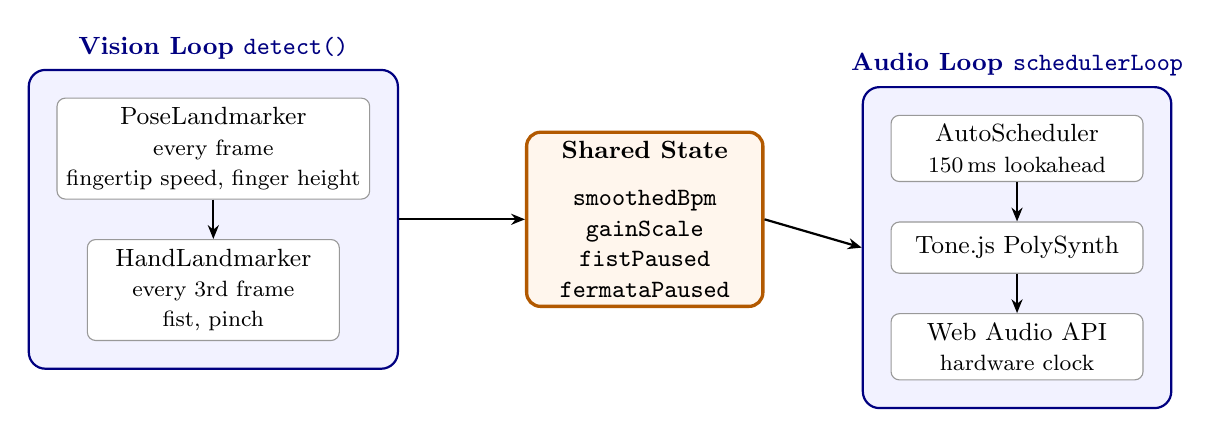
\begin{tikzpicture}[
  compbox/.style = {
    rectangle, draw=black!40, fill=white,
    rounded corners=3pt, align=center,
    minimum width=3.2cm, minimum height=0.65cm,
    font=\small},
  sharedbox/.style = {
    rectangle, draw=orange!70!black, fill=orange!7,
    very thick, rounded corners=5pt, align=center,
    minimum width=3.0cm, minimum height=1.8cm,
    font=\small},
  groupbg/.style = {
    rectangle, draw=blue!50!black, fill=blue!5,
    thick, rounded corners=6pt},
  arr/.style  = {-{Stealth[length=5pt,width=4pt]}, thick},
  lbl/.style  = {font=\footnotesize, fill=white,
                 inner sep=2pt, align=center}
]

%── Vision Loop nodes ────────────────────────────────────────────
\node[compbox] (PLM) at (0, 0.55)
  {PoseLandmarker\\{\footnotesize every frame}\\
   {\footnotesize fingertip speed, finger height}};

\node[compbox, below=0.5cm of PLM] (HLM)
  {HandLandmarker\\{\footnotesize every 3rd frame}\\
   {\footnotesize fist, pinch}};

\draw[arr] (PLM) -- (HLM);

%── Vision Loop background box ───────────────────────────────────
\begin{scope}[on background layer]
  \node[groupbg,
    fit=(PLM)(HLM),
    inner sep=10pt,
    label={[font=\small\bfseries, text=blue!50!black]
           above:Vision Loop \texttt{detect()}}] (VL) {};
\end{scope}

%── Shared State node ────────────────────────────────────────────
\node[sharedbox, right=1.6cm of VL.east] (SS)
  {\textbf{Shared State}\\[6pt]
   \texttt{smoothedBpm}\\
   \texttt{gainScale}\\
   \texttt{fistPaused}\\
   \texttt{fermataPaused}};

%── Audio Loop nodes ─────────────────────────────────────────────
\node[compbox, right=1.6cm of SS.east, yshift=0.90cm] (ASC)
  {AutoScheduler\\{\footnotesize 150\,ms lookahead}};

\node[compbox, below=0.5cm of ASC] (TJS)
  {Tone.js PolySynth};

\node[compbox, below=0.5cm of TJS] (WAP)
  {Web Audio API\\{\footnotesize hardware clock}};

\draw[arr] (ASC) -- (TJS);
\draw[arr] (TJS) -- (WAP);

%── Audio Loop background box ────────────────────────────────────
\begin{scope}[on background layer]
  \node[groupbg,
    fit=(ASC)(TJS)(WAP),
    inner sep=10pt,
    label={[font=\small\bfseries, text=blue!50!black]
           above:Audio Loop \texttt{schedulerLoop}}] (AL) {};
\end{scope}

%── Cross arrows ─────────────────────────────────────────────────
\draw[arr] (VL.east) -- (SS.west);
\draw[arr] (SS.east) -- (AL.west);

\end{tikzpicture}
\caption{System architecture of Air Conductor. Two independent
  \texttt{requestAnimationFrame} loops communicate exclusively through
  shared module-level state. The four state variables serve distinct
  roles: \texttt{smoothedBpm} carries the EWMA-filtered tempo estimate;
  \texttt{gainScale} carries the current note-velocity multiplier
  ($g \in [0.1,\,2.0]$); and \texttt{fistPaused} and
  \texttt{fermataPaused} are Boolean transport flags that halt or
  sustain playback, respectively. The audio loop derives beat timing
  solely from the Web Audio API hardware clock; MediaPipe inference
  latency in the vision loop cannot affect audio scheduling.}
\label{fig:architecture}
\end{figure*}

% ---------------------------------------------
%  IV. IMPLEMENTATION
% ---------------------------------------------
\section{Implementation}
\label{sec:impl}

\subsection{MIDI Analysis}

\texttt{MidiAnalyzer} parses a Standard MIDI File (SMF) binary in its
constructor. It extracts: the ticks-per-beat value \texttt{tpb} from
the SMF header (default 480); the initial tempo $T_{\mu s}$
(microseconds per beat) from the first \texttt{0xFF\,0x51} meta-event
(default 500\,000); and the time signature from the first
\texttt{0xFF\,0x58} meta-event. The initial tempo in beats per minute
(BPM) is:

\begin{equation}
  \text{BPM}_0 = \frac{60{,}000{,}000}{T_{\mu s}}
  \label{eq:bpm}
\end{equation}

Compound metres (6, 9, 12 beats) are mapped to simple equivalents
(2, 3, 4), and any remaining unsupported time signature is forced to
4/4. The parser collects a sorted array of note-on and note-off events
with absolute tick positions; percussion channel~9 events are parsed
but filtered at playback time.

\subsection{Audio Pipeline}

The audio signal chain is fixed for the lifetime of a file load:
\begin{align*}
  &\texttt{instrument},\;\texttt{fermataSustainSynth}\\
  &\quad\longrightarrow\;\texttt{fermataGain}
     \;\longrightarrow\;\texttt{Tone.Destination}
\end{align*}
Both \texttt{instrument} and \texttt{fermataSustainSynth} are
\texttt{Tone.PolySynth} instances configured with a
\texttt{fattriangle} oscillator---three detuned triangle waves (spread
20\,cents)---producing an organ timbre. The main \texttt{instrument} is
set at $-12\,\text{dB}$ with a near-zero 10\,ms attack, full sustain,
and a 300\,ms release, mimicking an organ key. The
\texttt{fermataSustainSynth} is set at $-20\,\text{dB}$ with a slower
150\,ms attack and a 400\,ms release; it is used exclusively during
fermata gestures to sustain captured chord tones while the main
instrument's voices decay (Section~\ref{sec:fermata}). Both synths
connect in parallel to a shared \texttt{Tone.Volume(0)} node
(\texttt{fermataGain}), which acts as a common output bus and is not
manipulated during normal playback. The file-load handler awaits
\texttt{Tone.start()} before presenting the start overlay.

The \texttt{AutoScheduler} advances a 150\,ms lookahead window each
\texttt{requestAnimationFrame} (rAF) frame. The beat interval in
seconds is:

\begin{equation}
  I = \frac{60}{\text{BPM}_0 \times f}
  \label{eq:interval}
\end{equation}

\noindent where $f = \texttt{smoothedBpm} / \texttt{BPM}_0$ is the
real-time speed factor from the beat detector
(Section~\ref{sec:beatdetect}). Each scheduled note fires at the
proportionally interpolated audio time within its beat interval and is
rendered via \texttt{triggerAttackRelease} with a fixed duration of
0.35\,s.

\subsection{Beat Detection and Tempo Modulation}
\label{sec:beatdetect}

At each pose-estimation frame, the right index-fingertip coordinate
$(x, y)$ (PoseLandmarker landmark 20, normalised $[0,1]$) is appended
to a circular buffer of length 8. Instantaneous speed is the mean
Euclidean displacement per millisecond across the $W-1 = 2$ consecutive
frame-to-frame pairs within a $W = 3$-frame sliding window:

\begin{equation}
  v = \frac{1}{n} \sum_{i=k-W+2}^{k}
      \frac{\sqrt{(x_i - x_{i-1})^2 + (y_i - y_{i-1})^2}}{\Delta t_i},
  \quad W = 3
  \label{eq:speed}
\end{equation}

\noindent where $n$ is the number of valid frame pairs
($0 < \Delta t_i < 100\,\text{ms}$), $n \leq W - 1 = 2$. A jump filter clears the buffer if the Manhattan distance
from the last sample exceeds $0.25$, discarding teleporting landmarks.

A per-hand two-state FSM (Fig.~\ref{fig:fsm}) detects each conducting
ictus. In the \textsc{Idle} state, the FSM transitions to
\textsc{Rising} when $v$ exceeds a sensitivity-dependent threshold:

\begin{equation}
  \theta = 0.003 \times 0.22^{\,(s-1)/4}, \quad s \in \{1,\ldots,10\}
  \label{eq:threshold}
\end{equation}

\noindent where $s$ is the user-configured sensitivity (default $s=1$,
$\theta = 0.003$; at $s=10$, $\theta \approx 9.94 \times 10^{-5}$). The base
value $\theta_0 = 0.003$ (normalised units per millisecond) and the
exponential base $0.22$ were determined empirically to span comfortable
conducting speeds---from slow adagio strokes at the default sensitivity
to rapid allegro gestures at maximum sensitivity---on commodity laptop
hardware. Higher $s$ lowers $\theta$, increasing responsiveness to
slower gestures. A fire event (ictus) is emitted when, in
\textsc{Rising}, the speed falls to 55\% of the observed peak:

\begin{equation}
  v < 0.55 \cdot v_{\text{peak}}
  \label{eq:fire}
\end{equation}

\noindent subject to: (a) the rising phase lasted $\leq 600\,\text{ms}$
(rejects slow drifts) and (b) $\geq 200\,\text{ms}$ have elapsed since
the previous ictus (prevents double-triggering within a single stroke).

\begin{figure*}[ht!]
  \centering
  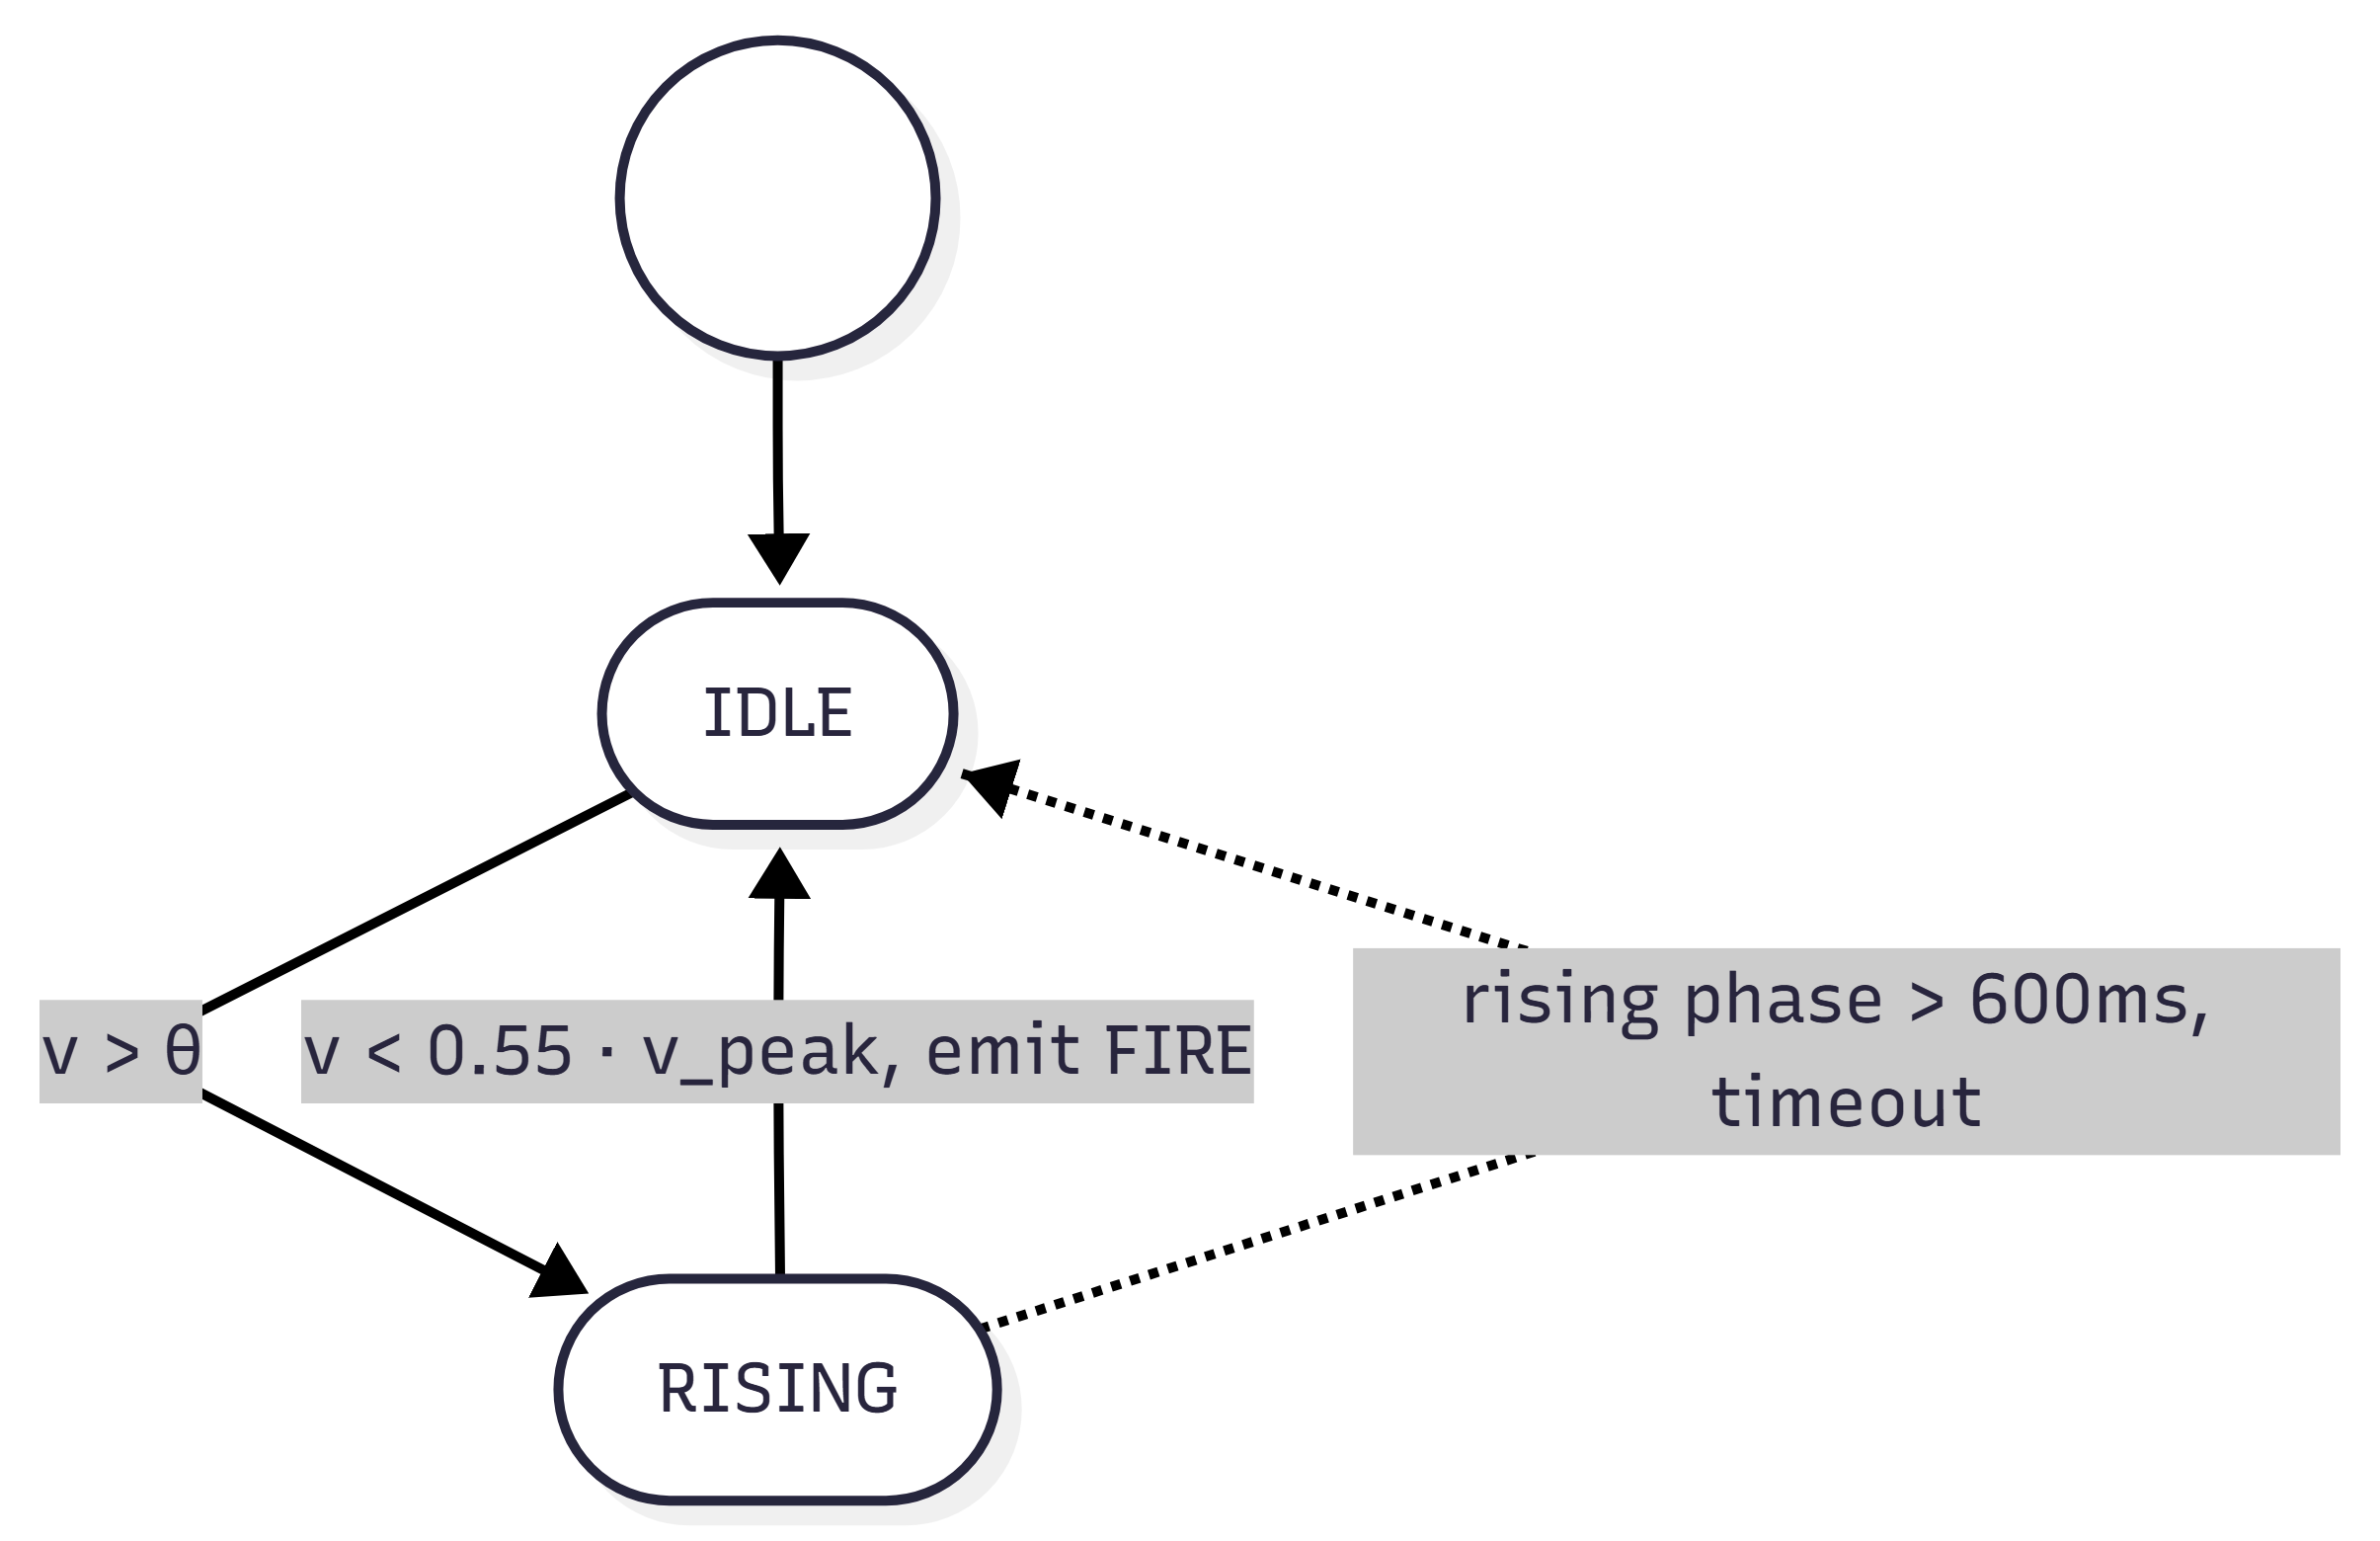
\includegraphics[width=0.55\textwidth]{fig_fsm}
  \caption{Per-hand gesture detection FSM for conducting stroke (ictus)
  detection. The FSM enters \textsc{Rising} when index-fingertip speed
  exceeds threshold $\theta$ and fires an ictus on the falling edge
  when speed drops to 55\% of the stroke peak. The 600\,ms timeout
  path rejects slow drifts without emitting a fire event; the 200\,ms
  inter-ictus guard prevents double-triggering within a single stroke.}
  \label{fig:fsm}
\end{figure*}

On each ictus, the inter-ictus interval $\Delta t_{\text{ictus}}$
yields a raw BPM estimate:

\begin{equation}
  \text{BPM}_{\text{raw}} = \frac{60{,}000}{\Delta t_{\text{ictus}}}
  \label{eq:raw_bpm}
\end{equation}

\noindent Inter-ictus intervals outside the range
$[200,\,3000]\,\text{ms}$ (corresponding to 20--300\,BPM) are
discarded without updating \texttt{smoothedBpm}. Otherwise,
$\text{BPM}_{\text{raw}}$ is clamped to
$[0.4 \cdot \text{BPM}_0,\; 2.5 \cdot \text{BPM}_0]$ and smoothed by
an exponential weighted moving average (EWMA):

\begin{equation}
  \text{BPM}_{\text{smooth}}
    \leftarrow 0.65 \cdot \text{BPM}_{\text{smooth}}
              + 0.35 \cdot \text{BPM}_{\text{clamped}}
  \label{eq:smooth}
\end{equation}

\noindent The speed factor $f = \text{BPM}_{\text{smooth}} /
\text{BPM}_0$ is immediately applied to the scheduler via
\texttt{setSpeed}($f$), updating the beat interval $I$ per
Equation~(\ref{eq:interval}). A rolling buffer of the last six raw
estimates also maintains an average BPM displayed in the HUD.

\subsection{Volume Control}

The left index fingertip (PoseLandmarker landmark 19) is tracked
relative to the left shoulder (landmark 11) and left hip (landmark 23).
At each pose-estimation frame, the gain scale $g \in [0.1,\,2.0]$ is
updated as:

\begin{equation}
  g_{t+1} = \begin{cases}
    \min(2.0,\; g_t + 0.01) & \text{if } y_{\text{finger}}
      < y_{\text{shoulder}} \\
    \max(0.1,\; g_t - 0.01) & \text{if } y_{\text{finger}}
      > y_{\text{hip}} \\
    g_t & \text{otherwise}
  \end{cases}
  \label{eq:gain}
\end{equation}

\noindent where smaller $y$ is higher on screen (MediaPipe normalised
coordinates). At a nominal frame rate of 60\,fps, the $\pm0.01$
per-frame step traverses the full gain range $[0.1,\,2.0]$ in
approximately 3.2\,s, consistent with the duration of a natural arm
raise or lower during expressive conducting. The gain is propagated to
\texttt{scheduler.gainScale} each frame and applied as a velocity
multiplier in note scheduling:
$v_{\text{note}} = (v_{\text{midi}}/127) \times 0.9 \times g$,
where the $0.9$ headroom factor prevents clipping at maximum gain $g = 2.0$.

\begin{figure*}[t!]
  \centering
  % ── Row 1 ──────────────────────────────────────────────────────
  \begin{subfigure}[t]{0.23\textwidth}
    \centering
    \includegraphics[width=\linewidth]{PANELA}
    \caption{Right-hand conducting stroke. Index-fingertip speed
    (PoseLandmarker lm[20]) modulates tempo via EWMA ($\alpha=0.35$).}
  \end{subfigure}\hfill
  \begin{subfigure}[t]{0.23\textwidth}
    \centering
    \includegraphics[width=\linewidth]{PANELB}
    \caption{Left hand above shoulder (lm[11]). Gain increments
    $+0.01$/frame toward $g=2.0$.}
  \end{subfigure}\hfill
  \begin{subfigure}[t]{0.23\textwidth}
    \centering
    \includegraphics[width=\linewidth]{PANELC}
    \caption{Left hand in neutral zone between shoulder (lm[11])
    and hip (lm[23]). Gain unchanged.}
  \end{subfigure}\hfill
  \begin{subfigure}[t]{0.23\textwidth}
    \centering
    \includegraphics[width=\linewidth]{PANELD}
    \caption{Left hand below hip (lm[23]). Gain decrements
    $-0.01$/frame toward $g=0.1$.}
  \end{subfigure}

  \vspace{0.8em}

  % ── Row 2 ──────────────────────────────────────────────────────
  \hspace*{0.12\textwidth}
  \begin{subfigure}[t]{0.23\textwidth}
    \centering
    \includegraphics[width=\linewidth]{PANELE}
    \caption{Left fist held $\geq$300\,ms triggers cut-off;
    playback resumes 800\,ms after hand opens. (HandLandmarker)}
  \end{subfigure}\hfill
  \begin{subfigure}[t]{0.23\textwidth}
    \centering
    \includegraphics[width=\linewidth]{PANELF}
    \caption{Left pinch held $\geq$20\,ms triggers fermata with
    chord sustain. (HandLandmarker)}
  \end{subfigure}
  \hspace*{0.12\textwidth}

  \caption{Four-gesture vocabulary. Red highlights the active
  landmark region. (a)--(d) use PoseLandmarker; (e)--(f) use
  HandLandmarker.}
  \label{fig:gestures}
\end{figure*}


\subsection{Fist Cut-Off}

The fist gesture is classified from \texttt{HandLandmarker} landmarks
of the left hand. A hand is classified as a fist when all four
fingertips are closer to the wrist (landmark~0) than their respective
metacarpophalangeal (MCP) knuckles:

\begin{equation}
  d(\ell_0, \ell_f) < d(\ell_0, \ell_{f-3}),
  \quad \forall f \in \{8,\,12,\,16,\,20\}
  \label{eq:fist}
\end{equation}

\noindent where $\ell_k$ denotes the $k$-th \texttt{HandLandmarker}
landmark and $d(\cdot,\cdot)$ is Euclidean distance in normalised
landmark space. A confirmed fist held for $\geq 300\,\text{ms}$ invokes
\texttt{scheduler.pause()} and \texttt{scheduler.\_stopAll()} (which
calls \texttt{releaseAll()} on the synthesiser), setting
\texttt{fistPaused = true}. Playback resumes 800\,ms after the hand
opens; this delay was determined empirically to allow the 300\,ms
synthesiser release envelope to fully decay and to provide a perceptible
pause before the next phrase begins.

\subsection{Fermata Pinch}
\label{sec:fermata}

A pinch is detected when the normalised thumb-tip to index-tip distance
falls below 25\% of hand size:

\begin{equation}
  \frac{d(\ell_4,\, \ell_8)}{d(\ell_0,\, \ell_9)} < 0.25
  \label{eq:pinch}
\end{equation}

\noindent A pinch held for $\geq 20\,\text{ms}$ induces a fermata. The
entry sequence is: (1) \texttt{scheduler.pauseOnly()}---which freezes
score advancement without invoking \texttt{releaseAll()}, so
currently-sounding notes continue to decay through their natural release
envelopes; (2) identify recently fired notes from
\texttt{scheduler.lastChord}---a
\texttt{Map$\langle$noteName, audioTime$\rangle$} accumulating all
note-on events---by selecting entries where
$t_{\text{sched}} \leq t_{\text{now}}$ and
$t_{\text{now}} - t_{\text{sched}} < \text{NOTE\_SUSTAIN}$, with
\begin{equation*}
  \text{NOTE\_SUSTAIN} = \max(0.6,\; I \times 1.2) \;\text{seconds};
\end{equation*}
the 0.6\,s lower bound ensures chord capture at tempos up to 100\,BPM,
where the beat interval $I$ falls below 0.6\,s and the $1.2 \times I$
term alone would be insufficient to capture recently triggered notes;
(3) if at least one note is captured, schedule a
\texttt{triggerAttack} on \texttt{fermataSustainSynth} at velocity~0.5
after a 150\,ms delay. The delay ensures the main instrument's onset
transient has fully passed before the sustain synth rises, preventing
the listener from perceiving two distinct note onsets. The sustain
synth's slower 150\,ms attack envelope and lower volume ($-20\,\text{dB}$)
cause it to emerge gradually beneath the still-decaying main synthesiser.

On pinch release there are two paths. If the pinch is released
\emph{before} the 150\,ms attack timer fires, the pending timer is
cancelled and playback resumes immediately with no sustain-synth
involvement. If the pinch is released \emph{after} the attack has
fired, \texttt{triggerRelease} is called on
\texttt{fermataSustainSynth}, whose 400\,ms release envelope provides a
smooth fade-out; playback resumes after a 450\,ms delay to ensure the
sustain-synth voice is fully silent before new MIDI notes begin,
preventing harmonic overlap between the fading fermata chord and
resumed playback.



\subsection{Heads-Up Display}

The HUD is rendered on a transparent HTML canvas element
(\texttt{hudCanvas}), an overlay whose buffer is sized to the
container's CSS layout dimensions scaled by
\texttt{window.devicePixelRatio} and kept in sync by a
\texttt{ResizeObserver}, driven by a third
\texttt{requestAnimationFrame} loop fully decoupled from both the audio
and vision loops. It shows:
(a) a beat-anticipation arc sweeping clockwise from 12\,o'clock,
driven by interpolation between the previous and next scheduled beat
times; (b) a radial flare emitted when the current time crosses the
scheduled beat time; (c) a beat-number label, highlighted for the
downbeat; (d) three BPM panels labelled \textsc{Score}, \textsc{Live},
and \textsc{Avg}, showing the score BPM ($\text{BPM}_0$), the current
smoothed BPM, and the rolling six-beat average, respectively; and
(e) a vertical dynamics bar reflecting the current gain $g$. All
colours are derived from CSS custom properties, keeping the HUD
consistent across light and dark themes.

\subsection{Font-Size Accessibility and Elder Display Mode}

The system provides a CSS-only font-size control that also serves as an
elder accessibility mode. A three-level selector (small, medium, large)
in the header sets the \texttt{data-fontsize} attribute on the
\texttt{<html>} element, persisted via \texttt{localStorage} and
restored before the first paint by an inline script. The attribute
drives CSS custom properties \texttt{--fs-label}, \texttt{--fs-body},
and \texttt{--fs-val} uniformly across all text elements.

The \texttt{large} tier additionally activates targeted CSS overrides
that enlarge all interactive and visual feedback elements: header
buttons (52$\times$52\,px), the sensitivity slider thumb
(30$\times$30\,px), the footer progress bar (8\,px height), and the
countdown numeral (14\,rem). The HUD renderer reads
\texttt{data-fontsize === "large"} each frame and responds by enlarging
the beat arc radius, the beat-number font, the wrist-dot radius
(11\,px vs.\ 6\,px), and the flare expansion distance. Because all
scaling is implemented purely through CSS attribute selectors and a
single in-JS conditional read---with no modification to gesture
thresholds, timing constants, or audio logic---the large tier provides
a complete elder accessibility profile within the same control as the
general font-size preference.

\subsection{Bilingual Interface}

The system provides a two-state language toggle (Traditional Chinese\,/\,English)
in the header. Activating the toggle sets the \texttt{data-lang}
attribute on the \texttt{<html>} element, persisted via
\texttt{localStorage} and restored before the first paint by an inline
script---following the same pattern as the font-size control. A
\texttt{setLang()} function iterates all elements tagged with
\texttt{data-i18n} (plain text) or \texttt{data-i18n-html} (rich text)
attributes and swaps their content from a static bilingual string table,
covering all visible interface text: header labels, help-panel
descriptions, overlay messages, and the canvas-rendered gesture
indicators (\textsc{Cut-off}, \textsc{Fermata}). The
\texttt{<html\,lang>} attribute is updated concurrently
(\texttt{zh-TW} or \texttt{en}) for screen-reader compatibility.
Gesture thresholds, timing constants, and audio logic are unaffected.

% ---------------------------------------------
%  V. DISCUSSION
% ---------------------------------------------
\section{Discussion}
\label{sec:discussion}

\subsection{Conducting Versus Playing Paradigm}

Removing pitch selection from the interaction loop reduces the
working-memory demand of the interface and broadens engagement across
musical experience and cognitive ability levels. A conductor need not
know individual note names---only how to express faster, slower,
louder, and softer---making the system accessible to users with any
level of musical training.

\subsection{Gesture Vocabulary Design}

The four-gesture vocabulary covers two levels of musical control. At
the macro level, tempo and volume are continuous channels modulated by
gross arm motion (index-fingertip speed, fingertip height), consistent
with evidence that large-movement interfaces reduce physical barriers for
elderly users~\cite{rw11,rw12}. At the note level, the fist cut-off
and fermata pinch correspond to standard conducting gestures: a sharp
closing of the fist signals an abrupt cut-off, and a sustained pinch
prolongs a held chord.

The deliberate assignment of discrete gestures (fist, pinch) to
\texttt{HandLandmarker} and continuous gestures (tempo, volume) to
\texttt{PoseLandmarker} reflects a hardware trade-off.
\texttt{HandLandmarker} provides the per-finger resolution needed for
fist and pinch classification but incurs higher inference cost. Running
it on every third frame reduces the per-frame budget by approximately
two-thirds relative to per-frame execution, while the 20\,ms and
300\,ms hold timers for pinch and fist respectively provide sufficient
temporal redundancy against frame-skipped detections.

\subsection{Decoupled Pipeline and Timing Accuracy}

A key reliability property of the architecture is that audio beat
timing cannot degrade under vision-pipeline load. Beat timestamps are
computed entirely from the Tone.js hardware clock and stored by
\texttt{schedulerLoop} before \texttt{detect()} reads them. Even if
the MediaPipe inference budget rises to 50\,ms per frame on a low-end
device, the 150\,ms lookahead buffer ensures that note events are
pre-scheduled and the audio subsystem continues unaffected.

\subsection{Limitations}

Several limitations of the current implementation warrant discussion.
First, beat detection uses only scalar index-fingertip speed; conducting
direction and pattern are not analysed, so no distinction is made
between 4/4 and 2/4 arm trajectories. Second, \texttt{MidiAnalyzer}
processes only the first tempo meta-event; mid-song tempo changes
(ritardando, accelerando) are silently ignored. Third, all MediaPipe
models and the Tone.js library load from external CDNs with no offline
fallback; network availability is a hard dependency. Fourth, the canvas
layout uses fixed pixel dimensions with no responsive breakpoints,
restricting use to landscape-oriented desktop browsers; portrait and
mobile viewports are not supported in the current release. Fifth, no
formal user study with elderly participants has been conducted;
accordingly, the accessibility and engagement claims in this paper rest
on the cited prior literature in Section~\ref{sec:related} rather than
on direct empirical evaluation of Air Conductor with the target
population, and the system's specific efficacy remains to be validated.

% ---------------------------------------------
%  VI. CONCLUSION
% ---------------------------------------------
\section{Conclusion}
\label{sec:conclusion}

We presented Air Conductor, a browser-native conducting simulator that
places the user in the role of an orchestral conductor over a MIDI
playback rendered by a Tone.js \texttt{PolySynth} organ synthesiser. A
four-gesture vocabulary and a decoupled dual-loop architecture provide
expressive musical control through only a standard webcam, with audio
beat timing governed by the Web Audio API hardware clock independent of
MediaPipe inference latency. A CSS-only three-level font-size control,
whose large tier serves as a complete elder accessibility profile,
and a bilingual (Traditional Chinese\,/\,English) interface toggle
together localise and scale the interface.

Future work will pursue: (1) directional stroke classification to
distinguish standard conducting beat patterns; (2) full MIDI tempo-map
parsing for ritardando and accelerando support; (3) offline asset
bundling via a service worker; and (4) a formal field evaluation with
elderly participants in community care settings.

% ---------------------------------------------
%  ACKNOWLEDGMENT
% ---------------------------------------------
\section*{Acknowledgment}
The authors thank the Department of Computer Science and Information
Engineering at National Chi Nan University for supporting this work.
This work was supported in part by the National Science and Technology
Council (NSTC), Taiwan, under Grant 114-2425-H-260-002-.

% ---------------------------------------------
%  REFERENCES
% ---------------------------------------------
\begin{thebibliography}{00}

\bibitem{rw1}
M. M. Wanderley and P. Depalle,
``Gestural control of sound synthesis,''
\textit{Proc. IEEE}, vol. 92, no. 4, pp. 632--644, Apr. 2004.

\bibitem{rw4}
B. Caramiaux, N. Montecchio, A. Tanaka, and F. Bevilacqua,
``Adaptive gesture recognition with variation estimation for
interactive systems,''
\textit{ACM Trans. Interact. Intell. Syst.},
vol. 4, no. 4, pp. 18:1--18:34, Dec. 2014.

\bibitem{rw5}
Z. Cao, G. Hidalgo, T. Simon, S.-E. Wei, and Y. Sheikh,
``OpenPose: Realtime multi-person 2D pose estimation using
part affinity fields,''
\textit{IEEE Trans. Pattern Anal. Mach. Intell.},
vol. 43, no. 1, pp. 172--186, Jan. 2021.

\bibitem{rw6}
Y. Chen, Y. Tian, and M. He,
``Monocular human pose estimation: A survey of deep
learning-based methods,''
\textit{Comput. Vis. Image Underst.}, vol. 192,
p. 102897, Mar. 2020.

\bibitem{rw8}
M. H. Thaut, G. C. McIntosh, and R. R. Rice,
``Rhythmic facilitation of gait training in hemiparetic stroke
rehabilitation,''
\textit{J. Neurol. Sci.}, vol. 151, no. 2,
pp. 207--212, Oct. 1997.

\bibitem{rw9}
T. S\"{a}rkam\"{o} \textit{et al.},
``Cognitive, emotional, and social benefits of regular musical
activities in early dementia: Randomized controlled study,''
\textit{Gerontologist}, vol. 54, no. 4, pp. 634--650, 2014.

\bibitem{rw10}
J. A. Grahn and M. Brett,
``Rhythm and beat perception in motor areas of the brain,''
\textit{J. Cogn. Neurosci.}, vol. 19, no. 5, pp. 893--906,
May 2007.

\bibitem{rw11}
L. H. Larsen, L. Schou, H. H. Lund, and H. Langberg,
``The physical effect of exergames in healthy elderly---a
systematic review,''
\textit{Games Health J.}, vol. 2, no. 4, pp. 205--212,
Aug. 2013.

\bibitem{rw12}
S. Wiemeyer and A. Kliem,
``Serious games in prevention and rehabilitation---a new
panacea for elderly people?''
\textit{Eur. Rev. Aging Phys. Act.}, vol. 9, no. 1,
pp. 41--50, 2012.

\bibitem{rw13}
P. Adenot and H. Choi,
``Web Audio API,'' W3C Recommendation,
World Wide Web Consortium, Jun. 2021. [Online]. Available:
\url{https://www.w3.org/TR/webaudio/}

\bibitem{rw14}
L. Wyse and S. Subramanian,
``The viability of the web browser as a computer music platform,''
\textit{Comput. Music J.}, vol. 37, no. 4, pp. 10--23,
Dec. 2013.

\end{thebibliography}

\end{document}